\documentclass[a4paper, 12pt]{article}
\usepackage[utf8]{inputenc}
\usepackage[T1]{fontenc}
\usepackage[margin=1.0in]{geometry}
\usepackage{graphicx}
\usepackage{listings}
\usepackage{hyperref}

\title{How2Use the Roculus Visualization for ROSIE.}
\date{2014-08-21}
\author{Daniel Bug}

\setlength{\parindent}{0pt}

\begin{document}
\maketitle

\section{Setting up ROSIE}
Here are the different steps to be done on the robot before the application start:
\begin{itemize}
\item Turn on the key and start-up robot base and computer.
\item When the login screen shows up, go into the EBC switch menu on the robot base and turn the last two 24.0V outputs ON. (7-0 and 7-1, 24V).
\item Switch on the sidekick computer by pressing the small red button at the side of the terminal.
\item Open a console and begin to start up the robot operating system. There is a startup script for a \emph{tmux} session that will have a set of all interesting terminals for you: \texttt{Ctrl+R 'start.sh' -> }. It takes a while to start teh first time. The first terminal is a display of the running processes (htop) and you can browse the terminals by using \texttt{Ctrl+b, n} or \texttt{Ctrl+b, p} to get to the next/previous terminal.\\ The following things need to run:
  \begin{itemize}
  \item \texttt{rosie\_core}
  \item \texttt{rosie\_robot}
  \item \texttt{rosie\_navigation} (You will probably have to init the navigation in rviz manually to have to robot localized correctly.)
  \item \texttt{rosie\_head\_camera}, which needs to be run on the sidekick. (Check that the terminal is an ssh session on the strands-sidekick, before you start the camera launch file).
  \end{itemize}
\item The application does not listen to the pure camera topics, but - in order to save bandwidth - relies on topics that are republished from a \emph{drop} node (\texttt{Ctrl+R 'drop'}):
  \begin{itemize}
  \item Open a new (tmux) terminal by typing \texttt{Ctrl+b, c}
  \item drop-node for the rgb images: \texttt{rosrun topic\_tools drop \\/head\_xtion/rgb/image\_color/compressed 9 10 \\/head\_xtion/rgb/image\_color/reducedBW/compressed \&}
  \item drop-node for the depth images: \texttt{rosrun topic\_tools drop\\ /head\_xtion/depth/hw\_registered/image\_rect/compressedDepth 9 10 \\/head\_xtion/depth\_registered/image\_rect/reducedBW/compressedDepth \&}
  \end{itemize}
The \texttt{9 10} parameters indicate that we will drop 9 out of 10 images, which will give around 3 fps for the video stream. You can work with higer values, but there will be a limit at which you start trading off a better frame rate against the position and orientation updates. For dropping 2/3 e.g. the images might take to much bandwidth for the transforms to be updated regularly and the stream will look nice, but appear at the wrong place.\\
The topics should print a notification on the terminal saying that they are advertising the new topic. If you don't see the message the head camera was probably not started correctly. There might be a short-cut, but I used to kill all terminals and launch everything from scratch again.
\end{itemize}

\section{Starting the Application}
Roculus relies on the folder structure. During start-up the roculus directory will be searched for multiple config files and map-components. They are explained in the next section.
\begin{itemize}
\item To start the application:
  \begin{itemize}
  \item On the visualization PC, make sure you are connected to rosienet and that your \texttt{/etc/hosts} file lists the correct IP adresses.
  \item Check with \texttt{echo \$ROS\_MASTER\_URI} that this environment variable is pointing to the robot, i.e.\ \texttt{http://scitosstrands:11311}
  \item If you want to use the gamepad launch the teleoperation node in a separate terminal:\\\texttt{roslaunch scitos\_teleop teleop\_joystick.launch}
  \item Go to the roculus folder: \texttt{roscd roculus}
  \item Start roculus: \texttt{rosrun roculus roculus\_node}, the start-up time can be in minutes, if the program is loading multiple room scans into the environment. (You can check the terminal output. To get there use \texttt{Alt+Tab}).
  \end{itemize}
\end{itemize}

\section{Configs, Resources and Map Data}
As mentioned there are several configs and resources used by the application:
\begin{itemize}
\item ogre.cfg: contains the screen and render settings for ogre, if this file can not be read, ogre will show a config dialog to recreate such a file.
\item plugins.cfg: specifies the plugins that will be loaded on start-up. Probably just the cg and particle library is needed, the rest will be commented out.
\item resources.cfg: points to the materials/textures/shaders for the game:
  \begin{itemize}
  \item media/sibenik.zip: one image from this archive is used as default initialization for textures
  \item media/rosie.zip: everything for the robot avatar
  \item media/game.zip: everything for the game... meshes for the keys/treasure/locks, their materials, etc.
  \item media/vertexColor.material: contains the materials for the thesis application, (blank material, video stream texture, snapshot texture)
  \item media/projection3D.cg: the cg shader programs that actually perform the reprojection from camera geometry to 3D snapshot. The color transformation for the sepia look if defined here as well.
  \end{itemize}
\item map directory: using the simpleXMLparser from Rares and the multiroom parser, all patrol-recordings in this folder are loaded into the environment during start-up
\item game.cfg: the configuration of your game environment. How many waypoints, how many keys, what are the rooms/corridors, which waypoints can be used for keys/locks/etc. Take a look at the comments inside the file.
\end{itemize}

\section{Functions on the Keyboard}
The keyboard will be used as a supervisor input. It can:
\begin{itemize}
\item ESC (3 times): End the application
\item i: reinitialize the game
\item p: toggle first person mode
\item a,d,s,w,(arrows), PgUp, PgDn: Move around in the world in free view
\item SPC: select a navigation target
\item m: toggle visibility of the map
\item v: toggle the visibility of the preloaded environment
\item F3: toggle visibility of the frame rate display
\item F4: toggle visibility of the application info display
\end{itemize}

\section{Functions on the Gamepad and Mouse\\(Player Input)}
The mouse can only select navigation targets by clicking (the selection still involves looking at the waypoint).\\
The gamepad has 4 possible functions:
\begin{itemize}
\item buttons 1-4: select a navigation target
\item button 8: reset the oculus orientation to look in the direction of the robot
\item cross-joystick (x-direction): look 120deg behind you (to the left/right)
\item only if the supervisor unmouted the player from first-person: you can fly around with the joysticks (left: forward+backward/turn, right: up+down and step left/right)
\end{itemize}
If another gamepad than the Logitec Rumble Pad is used, it will very likely be necessary to adapt the axis/button settings in BaseApplication::joyCallback(...), and PlayerBody::injectROSJoy(...). 

\section{Creating a new Scenario (Map)}
The default for now is the CVAP institute's map on floor 6, but eventually it can be necessary to get the robot running in a different environment.  Here're the changes that will effect the application: Roculus listens to the map topic and the interactive-marker topic on the robot to get the information for navigation and the environment is load from the recordings.  The obvious first steps are therefore to scan the new map with the robot and place the waypoints needed.  Furthermore, the surrounding has to be recorded as point clouds using the PTU. The resulting '.pcd' files will \emph{replace} the files in the map folder (save them in a different directory as backup).\\
For the application it is essential that at least the '[GAME]' section in the game.cfg file reflects the map correctly. The application should still start if you do not define any rooms, but if the number of waypoints does not match reality it might crash. Furthermore, I currently see a problem if you try to initialize a game (pressing 'i'), while the game.cfg specifies more keys than the number of rooms-1 (one room must be used for the treasure).\\
The way you can define rooms is quite easy: you just list the waypoint numbers that belong to the room. In addition, you need to declare at least one of them as a 'WP2Use'.  Door and DoorEvt together are used to place the virtual door (half way between the nodes).  The door waypoint can be a WP2Use at the same time.  The door event 'DoorEvt' must \emph{not} belong to the room (otherwise, it would be deactivated if the treasure is placed in this room and the game could therefore never be finished, since you can not trigger the door event).\\
Corridors are areas never to be used for game objects, specifying them should be optional, since the application parses them, but does not use them for the locig right now.\\ Take a look at the game.cfg comments as well to understand the setup better.  In \autoref{fig:minigame} you see the minimum setup of a game.

\begin{figure}[h!]
  \centering
  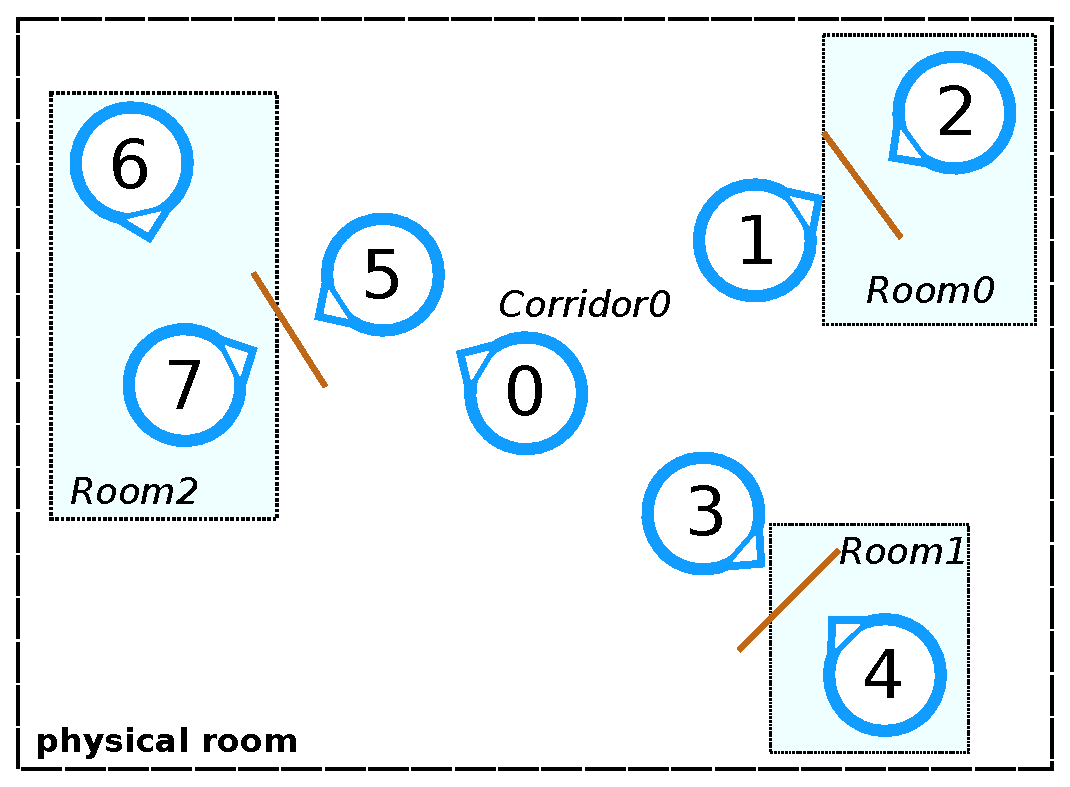
\includegraphics[width=0.7\textwidth]{./minigame.pdf}
  \caption{Minimalistic game setup: With one room for the treasure and up to two keys. This setup indicates that the rooms can be virtual areas in one physical room.}
  \label{fig:minigame}
\end{figure}

\bigskip
The corresponding game.cfg would look like this:
\begin{lstlisting}
[Game]
initWP = 1        #in case you want to use this -> BaseApplication 'i'
cntKeys = 1       #logical limit is 2 for this example
cntCorridors = 1  #index 0
cntRooms = 3      #indices from 0..2
cntWayPoints = 8  #indices from 0..7

[Corridor0]
WPs = 0 1 3 5

[Room0]
WPs = 2
WPs2Use = 2
Door = 2
DoorEvt = 1

[Room1]
WPs = 4
WPs2Use = 4
Door = 4
DoorEvt = 3

[Room2]        #the rooms on floor6 usually have this setup
WPs = 6 7
WPs2Use = 6
Door = 7
DoorEvt = 5
\end{lstlisting}

\section*{Contact}
Questions? Ask me:\\
Name: Daniel Bug\\
eMail: bug@kth.se\\

Code: github.com/dbug24/roculus, branch tekniskaDemo

\end{document}
